\begin{frame}{Master Motor (Left)}
  \framesubtitle{Setpoint and Response}
	\begin{itemize}
		\item Winds the metal strip $\Rightarrow$ Higher velocity (elongation)
		\item Dynamic model: $LM(s) \simeq \frac{5.398}{3.642S+1}$
	\end{itemize}
	\centering
	\includegraphics[width=1.00\textwidth]{identification_step_setpoints.png}
	\end{frame}


\begin{frame}{Master Motor}
  \framesubtitle{Controller Design}
	\begin{block}{PI Controller}

		\begin{itemize}
			\item Zero steady state error
			\item Disturbance rejection
			\item $\frac{K_i}{K_p} =$ chosen at $0.294$ to cancel plant pole
		\end{itemize}
	\end{block}
\end{frame}

\begin{frame}{Master Motor}
\framesubtitle{Tuning result}
\centering
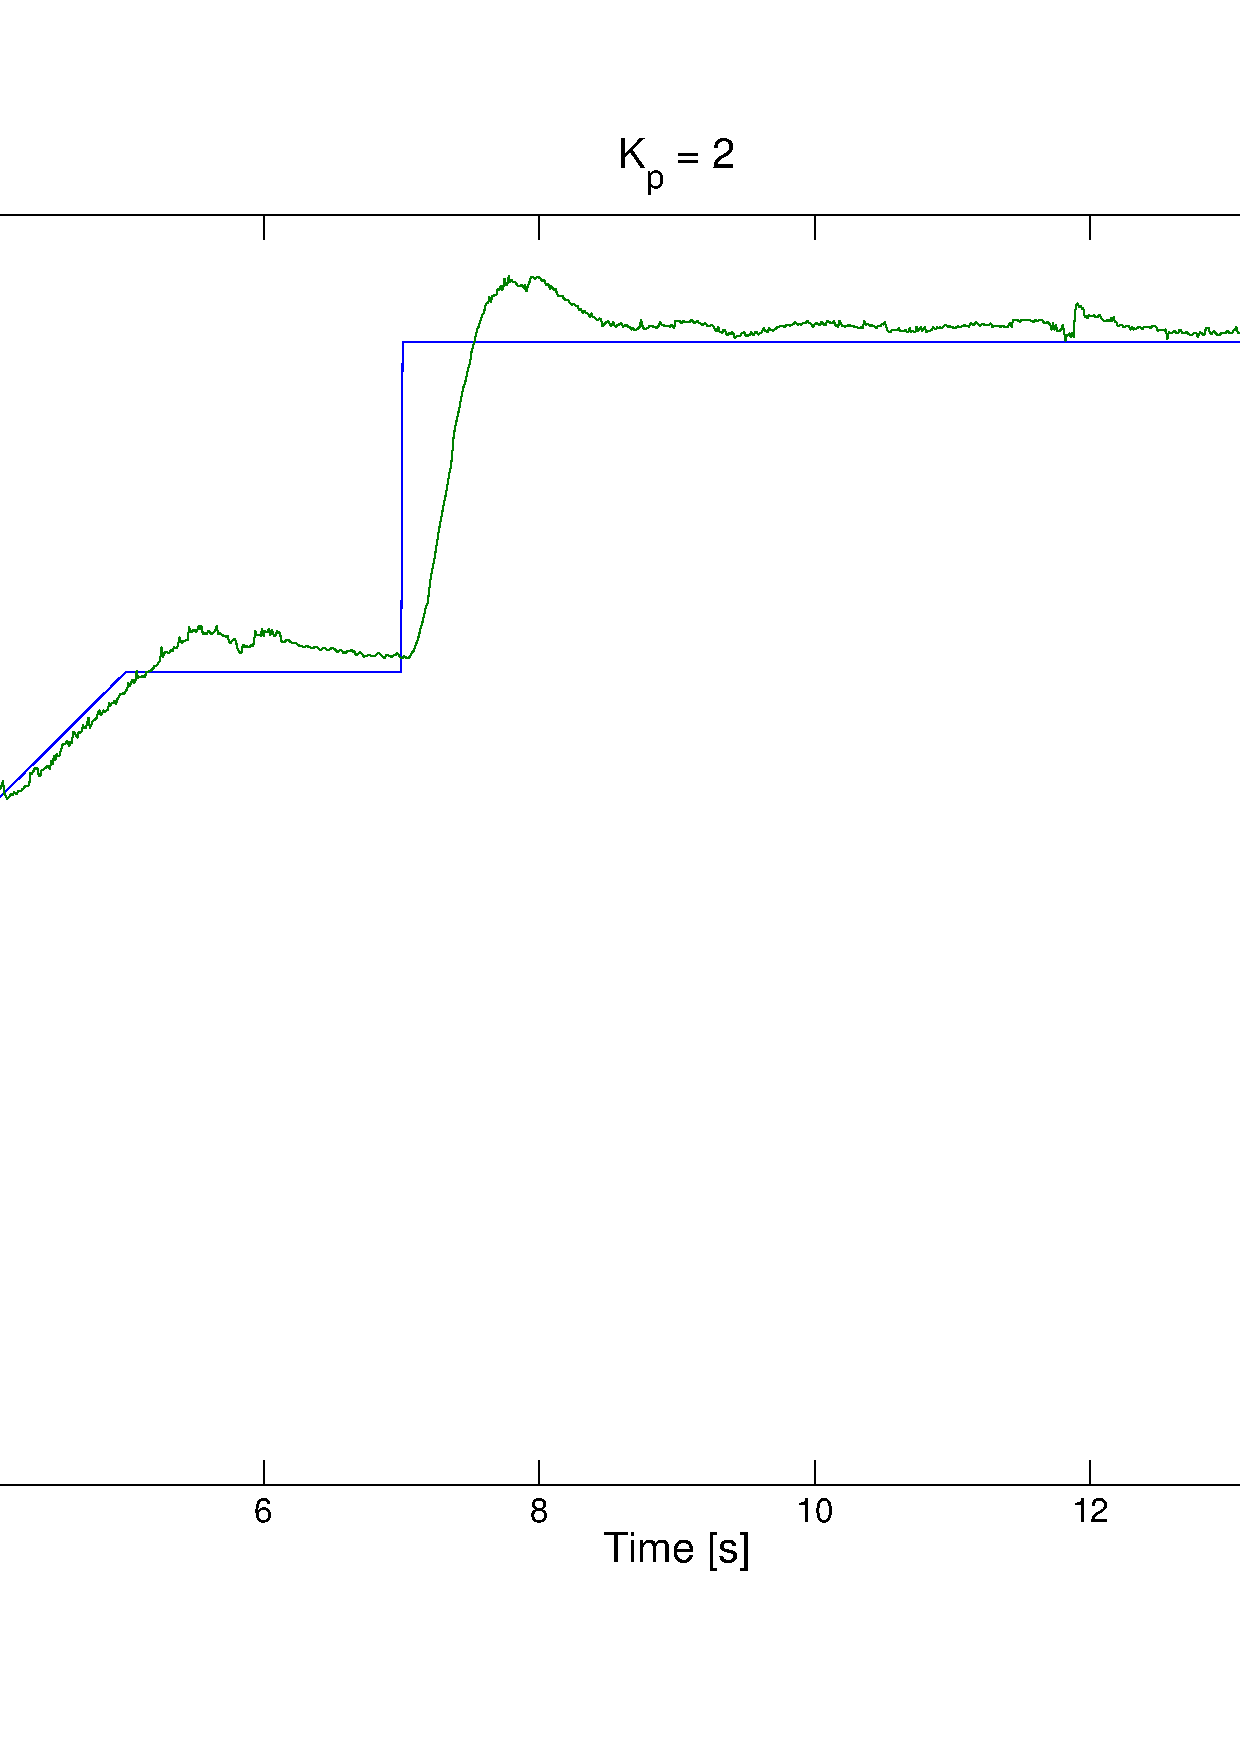
\includegraphics[width = \textwidth]{LM_KP200.pdf}
\end{frame}

\begin{frame}{Master Motor}
\framesubtitle{Conclusion}
\begin{itemize}
\item PI Controller for zero steady state error
\item Gain $K_P = 2$, $K_I = 0.588$ chosen for quickest settling time, reasonable overshoot
\item Overshoot is due to non linearities and higher order effects
\end{itemize}
\end{frame}
